\documentclass[12pt]{article}
\usepackage[utf8]{inputenc}  
\usepackage[francais]{babel}  
\usepackage{graphicx}
                 
\title{Architecture}             
\author{
	David Cheminade
	\and
	Guillaume Desbieys
	\and
	Quentin Michaud
	\and
	Hubert Mondon
}                       
\date{}
                            
\begin{document} 
	\maketitle{}                             

	\section{Diagramme de classes}    

		\subsection{Schéma UML}

			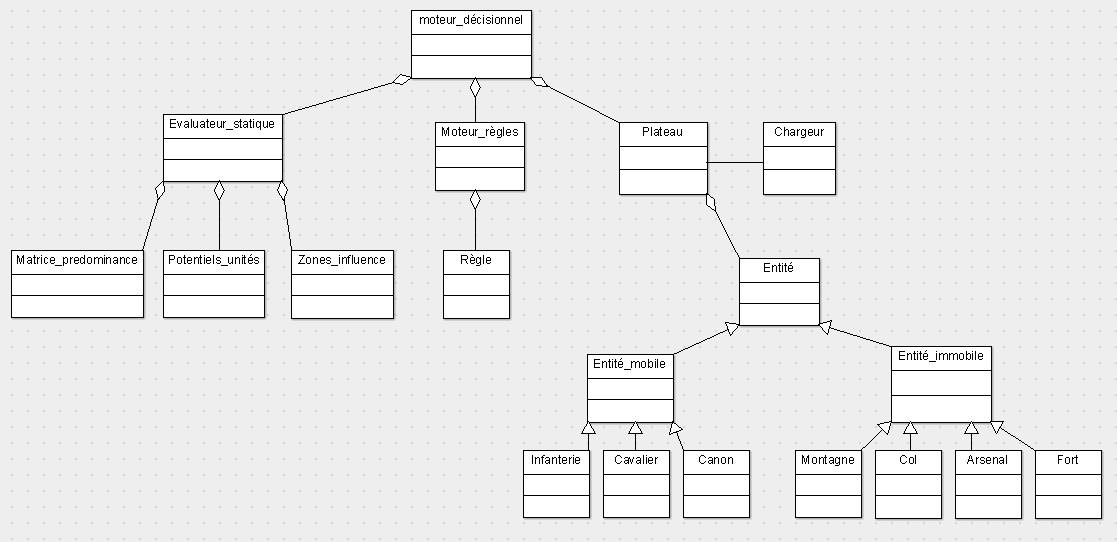
\includegraphics[scale=0.4]{images/diag_classes.jpg}

			\clearpage

		\subsection{Description des classes}

			\subsubsection{Plateau}
			
				\paragraph{Définition :}

				Le plateau est une matrice de taille fixe représentant une situation de jeu.

				\paragraph{Interaction :}

				Certaines cases du plateau contiendront des objets de type Entité.
				

			\subsubsection{Chargeur}

				\paragraph{Définition :}

				Classe permettant de charger une partie à partir d'un fichier. Elle transcrira les informations brute du fichier en un Plateau contenant des Entités.

				\paragraph{Interaction :}

				Le chargeur interagira avec le plateau puisque sa fonction consiste à modifier celui-ci.

			\subsubsection{Entité}

				\paragraph{Définition :}

				Les entités représentent les éléments de jeu. Sans entité, le plateau serait vide.

				\paragraph{Interaction :}

				Toutes les Entités seront disposées à l'intérieur d'une matrice dans la Classe Plateau.

			\subsubsection{Entité mobile}

				\paragraph{Définition :}

				Les entités mobiles sont les unités "jouables" telles que les infanteries, les cavaliers, les canons ou toute autre unité qu'il est possible de déplacer.

				\paragraph{Interaction :}

				Les Entités mobiles seront disposées à l'intérieur d'une matrice dans la Classe Plateau.

			\subsubsection{Entité immobile}

				\paragraph{Définition :}

				Les entités immobiles sont des entités présentes sur le plateau mais que les règles ne permettent pas de déplacer. Les forts, les arsenaux, les montagnes ou les cols sont par exemple des entités immobiles.

				\paragraph{Interaction :}

				Les entités immobiles seront disposées à l'intérieur d'une matrice dans la Classe Plateau. Certaines entités immobiles pourront par ailleurs contenir des entités mobiles. (exemple : les forts)

			\subsubsection{Moteur de règles}

				\paragraph{Définition :}

				Le moteur de règles est la classe qui se chargera de vérifier et de faire appliquer les règles du jeu qui lui seront données.

				\paragraph{Interaction :}

				Le moteur de règles intéragira avec le moteur décisonnel pour que celui-ci puisse choisir des coups valides et respectant les règles du jeu.

			\subsubsection{Règle}

				\paragraph{Définition :}

				Une règle sera une expression logique associée à un fait. Elles ne seront en fait pas codées sous forme de classe mais sous forme de fichier en ".drl".

				\paragraph{Interaction :}

				Les règles seront envoyées au moteur de règles qui devra se charger de les appliquer.

			\subsubsection{Zones influence}

				\paragraph{Définition :}

				Cette classe permettra de stocker l'ensemble des zones d'influences calculées par nos algorithmes, c'est à dire l'ensemble des cases sur lesquelles chaque unité peut agir.

				\paragraph{Interaction :}

				L'évaluateur statique se chargera de calculer les zones d'influences. Le moteur décisionnel s'en servira pour prendre la décision du coup à jouer.

			\subsubsection{Potentiels unités}

				\paragraph{Définition :}

				Cette classe permettra de stocker l'ensemble des potentiels offensifs et défensifs des unités en fonction de leur configuration spatiale.

				\paragraph{Interaction :}

				L'évaluateur statique se chargera de calculer les potentiels offensifs et défensifs. Le moteur décisionnel s'en servira pour prendre la décision du coup à jouer.

			\subsubsection{Matrice prédominance}

				\paragraph{Définition :}

				Cette classe permettra de stocker la matrice coefficientée de prédominance représentant les endroit avantageux ou à éviter.

				\paragraph{Interaction :}

				L'évaluateur statique se chargera de calculer la matrice. Le moteur décisionnel s'en servira pour prendre la décision du coup à jouer.

			\subsubsection{Evaluateur statique}

				\paragraph{Définition :}

				L'évaluateur statique est la classe permettant de calculer et stocker l'ensemble des résultats de nos algorithme d'évaluation statique du jeu.

				\paragraph{Interaction :}

				L'évaluateur statique agit directement sur "Zones influence", "Potentiels unités" et "Matrice predominance" puisqu'il se charge de les mettre à jour. Le moteur décisionnel aura quant à lui accès à l'évaluateur pour pouvoir prendre des décisions en fonction des résultats trouvés par l'évaluateur.

			\subsubsection{Moteur décisionnel}

				\paragraph{Définition :}

				Le moteur décisonnel se charge de choisir le coup à jouer en fonction d'une situation de jeu donnée et des résultats de l'évaluation statique.

				\paragraph{Interaction :}

				Le moteur décisionnel interagira avec le plateau pour connaître la situation de jeu, le moteur de règles pour jouer un coup valide, et l'évaluateur statique afin de se servir des résultats des algorithmes pour la prise de décision.





\end{document}                                 
